The digital system as a whole consists of several parts, mainly the control block, the ADC's and the clock pulse generator.The clock pulse generator creates a clock signal at $1 \mskip3mu KHz$, which is being used as a synchronizer clock signal for the control block.
This project only deals with the control block.

The digital control system is designed as a finite state machine with the states illegal, idle, expose and readout as shown in figure~\ref{fig:fsmDiagram}.
The logic connected to each state is as below.

\begin{outline}
  \1 Illegal
  \2 This state is mainly used for resets, it resets all peripherals and set the next state to idle.
  \1 Idle
  \2 This is the normal operating state, the machine always return to this state eventually.
  \2 In this state exposure increase and exposure decrease are enabled, increase takes presidence over decrease.
  \1 Expose
  \2 The machine normally stays in this state until the exposure time has passed.
  \2 Reset is the only working input.
  \1 Readout
  \2 The readout sequencer is started, the next state is set to idle afterwards.
  \2 Reset is the only working input.
\end{outline}

\begin{figure}[p]
  \centering
  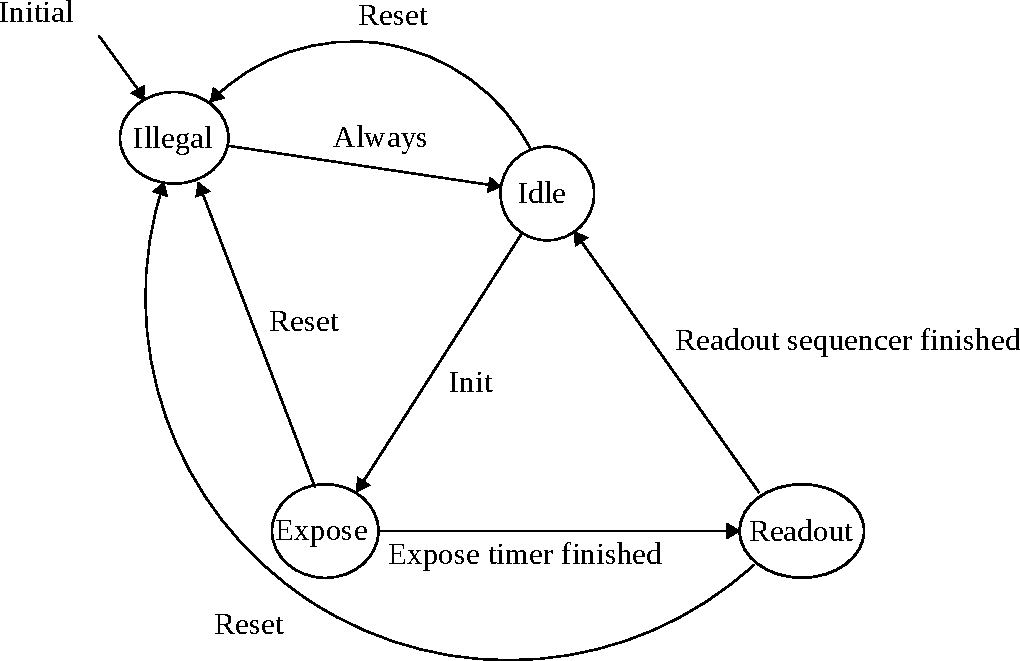
\includegraphics[width=0.85\textwidth]{figures/fsmDiagram}
  \caption{FSM representation of the digital control system}
  \label{fig:fsmDiagram}
\end{figure}

The main concern in the implementation of the hardware was maintainability since the project is meant as a proof of concept and not a production ready design.
The hardware was implemented as shown in more detail in figure~\ref{fig:digschematic}.
The countdown logic for the exposure was divided into two parts, one 5-bit register to store a value between 2 and 30 as well as a countdown register
to signal the end of the exposure period.

The readout cycle was also split out into its own sequencer independent of the rest of the machine.

\begin{figure}[p]
  \centering
  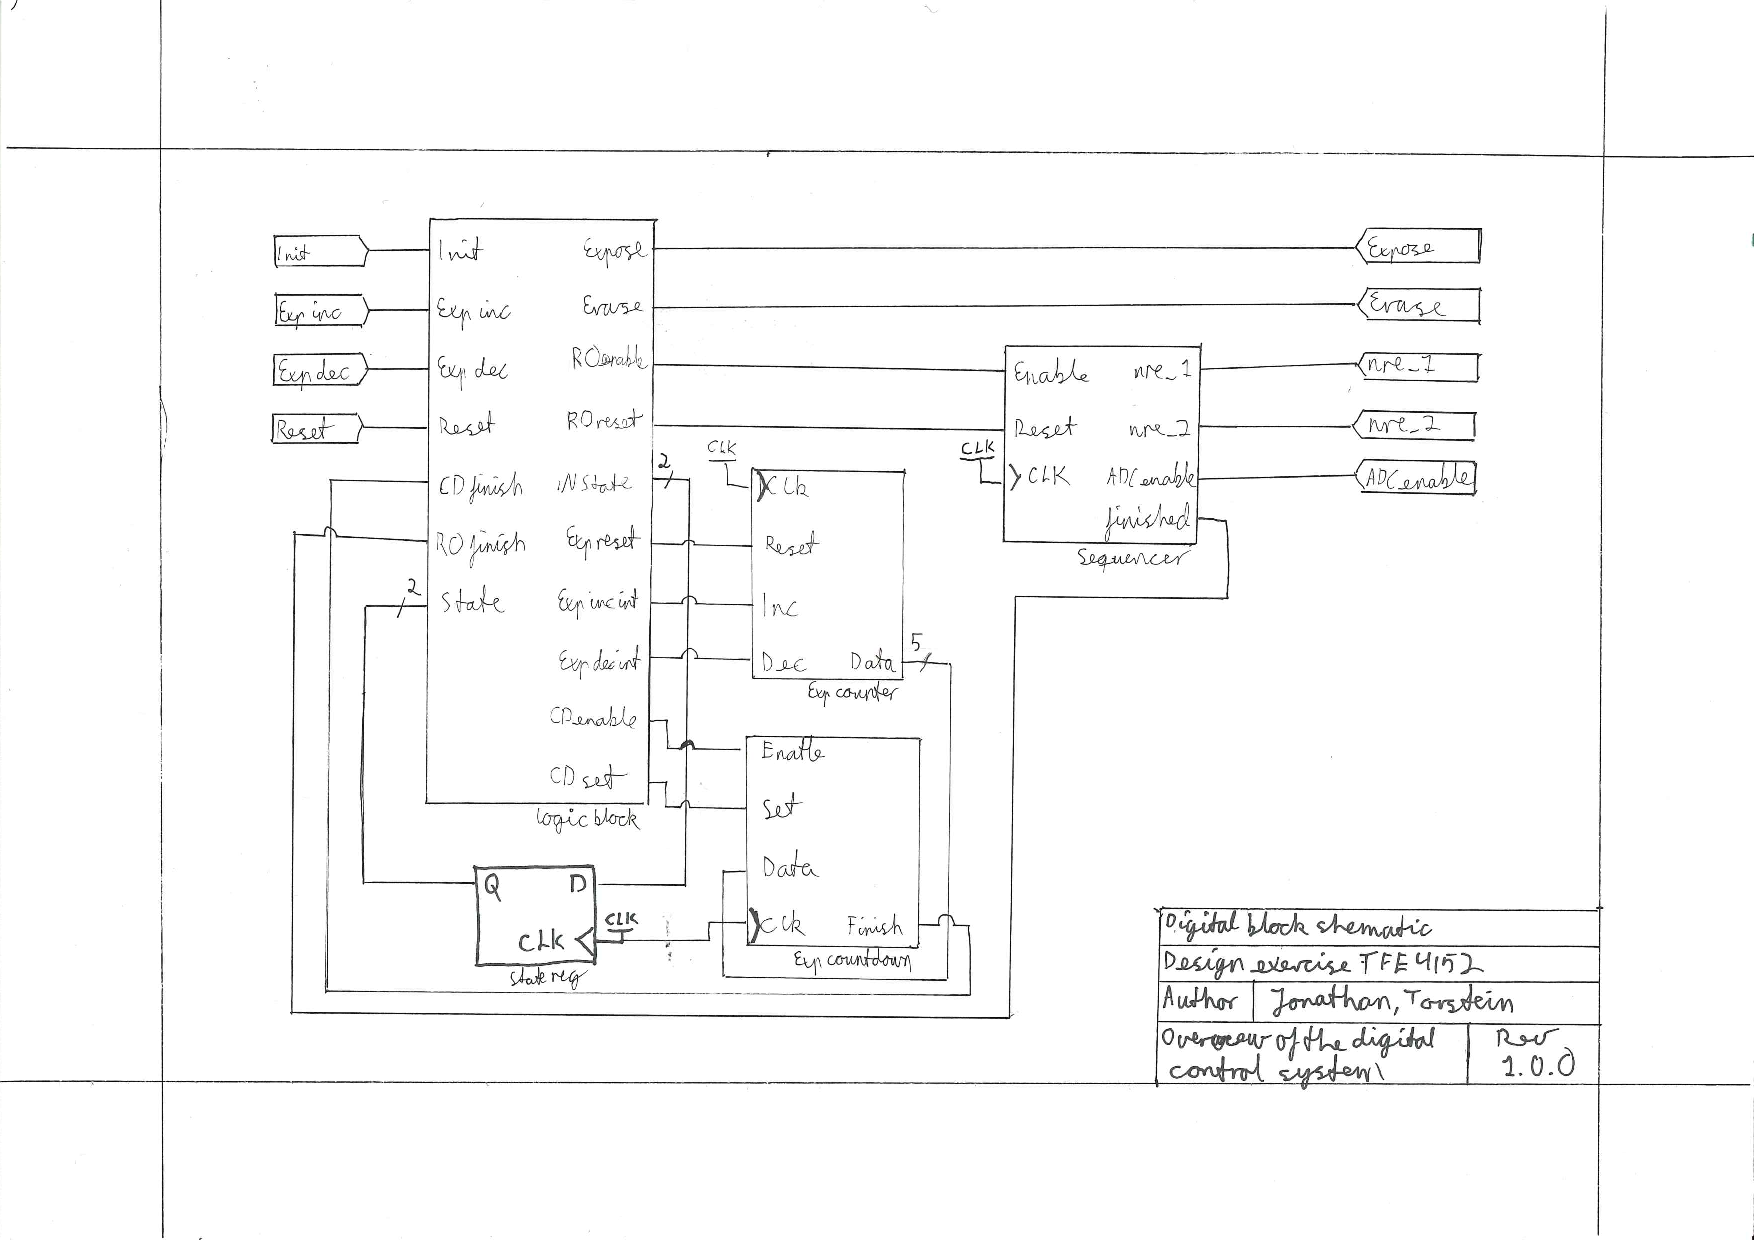
\includegraphics[width=0.85\textwidth]{figures/SchematicDigital}
  \caption{Schematic of the digital design, figure also found in Appendix~\ref{ap:Schematics}}
  \label{fig:digschematic}
\end{figure}

The full logical description of the digital control system is given in SystemVerilog 2012 in Appendix~\ref{ap:VerilogCode} along with simple test benches for the various components.
The design was heavily inspired by the FSM examples from~\cite{DigitalBook}.